\chapter{Time-memory-data tradeoff using rainbow table}
\label{chapter:tmdto-rainbow}

\indent \textbf{\textit{Summary.}} We introduce rainbow tables in this chapter. Rainbow tables have been proposed for block ciphers, as an improvement over Hellman tables. In order to use rainbow tables for stream ciphers, we derive a general tradeoff equation by taking $D$ into account. Then implementation is described and results obtained by varying the parameters are presented. Further, we derive a time-memory-data tradeoff equation on the lines of the Biryukov and Shamir tradeoff for Hellman tables. Towards the end, a comparison is done between these two tradeoff equations by using same tradeoff parameters.

\section{Rainbow table for block ciphers}
\label{sec:rainbow-block}

Rainbow table was introduced by Philippe Oechslin in \cite{oechslin:mfc}. Rainbow table (or rainbow chains, as called by the author) is a different way of precomputing data for the attack phase of a TMTO attack. Oechslin introduced rainbow table for block ciphers as an improvement over the Hellman tables. By using rainbow table, the attack time is expected to be reduced by a factor of $2$.

In Hellman tables, merging of chains within different tables is prevented by using different reduction functions for each table. However, collisions within the same table cannot be avoided completely. Though the number of elements in each table is restricted according to the table stopping rule, still there is no guarantee that collisions would not occur in the same table. This is due to the fact that birthday paradox is probabilistic in nature. Rainbow table solves this problem of collisions considerably.\\

\noindent \textit{\textbf{Precomputation phase.}} The rainbow table comprises of one huge table instead of $t$ tables, with $mt$ chains each having $t$ keys. The more interesting difference from Hellman tables is that instead of changing reduction function with table, reduction function is changed between columns of the table. If $SP_i$ is the starting point of a chain, then subsequent keys are computed by the functions \mbox{$f_1, f_2, \ldots, f_t$}, where $f_i(K) = R_i(E_{K}(P))$ for $1 \leq i \leq t$. This is shown in the following equations. 

\begin{align*}
& & K_{j,0} & = SP_j & & & &\\
1&. &K_{j,1} & = f_1(K_{j,0}) & & & &\\
2&. &K_{j,2} & = f_2(K_{j,1}) & & & &\\
& & &\vdots & & & &\\
(t-1)&. &K_{j,t-1} & = f_{t-1}(K_{j,t-2}) & & & &\\
(t)&. &K_{j,t} & = f_t(K_{j,t-1}) & & & &\\
& & EP_j & = K_{j,t} & & & &\\
\end{align*}

For every chain, the same sequence of mapping functions from $f_1$ to $f_t$ are used in computing subsequent keys. As usual, the starting and end points for each chain are stored in a hashtable, with the end points as the hashkey and the starting points as the hashvalue. The rainbow table is shown in figure \ref{fig:rainbow-table} (figure taken from \cite{oechslin:mfc}).

\begin{figure}[ht!]
	\centering
		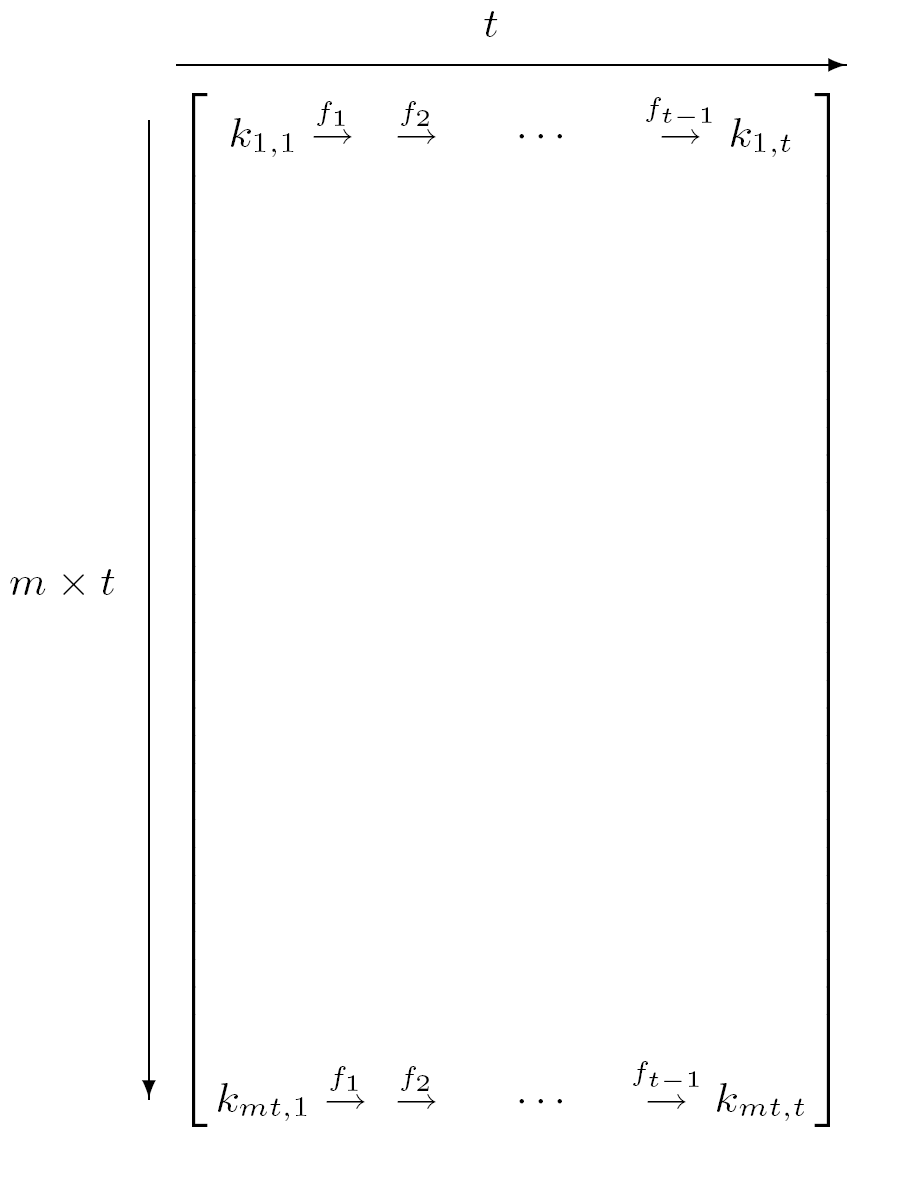
\includegraphics[width=3.5in]{./figures/rainbow-table.PNG}
	\caption{Rainbow table for block ciphers \cite{oechslin:mfc}}	
	\label{fig:rainbow-table}
\end{figure}

The time for preparing the rainbow table is the same as the number of computations carried out. This is equal to $P$ = $mt \times t$ = $mt^2$. Also, the order of memory required for the hash table is $M$ = $mt$. \\

\noindent \textit{\textbf{Attack phase.}} The attack phase is a little more complicated as compared to that for Hellman tables. But, as we shall see, in the worst case the number of computations required to find a match is reduced by a factor of $2$. 

First, let's consider the possibility of the ciphertext appearing in the last column of the rainbow table. If this is the case, then an end point $EP_j$ must match the reduction of $C$ which is $X$ = $R_t(C)$. Note that the reduction function for the $t$'th column is used here. Once the match occurs, $(t-1)$ computations using the mapping function are performed starting from the corresponding starting point $SP_j$, with the mapping function changing in each column. $K_{j,t-1}$ is then the required key, if it is not a false alarm. However if the match does not occur, the number of computations is 0, as the mapping function is never called for $X$.

Next, the possibility of $C$ appearing in the $(t-1)$'th column is explored. $X$ is computed as $X = f_{t}(R_{t-1}(C))$ and compared with the end points. If there is a match, then $(t-2)$ computations are performed from $SP_{j}$ using the mapping functions $f_1, f_2, \ldots, f_{t-2}$. The key computed is $K_{j,t-2}$ which is the required key. But if there is no match, the number of computations performed for $X$ is just $1$.

This process is repeated for all the columns. In the worst case scenario, $C$ appears in the second column of the table (which is the last possibility). In this case, the mapping functions $f_2, f_3, \ldots, f_t$ are used in sequence to compute $X$, taking a total of $(t-1)$ computations. After $X$ matches with $EP_j$, the required key is $K_{j,0}$ or $SP_j$. 

The total number of computations performed before the key is found is the sum of computations done for checking $C$ in all the columns, and is,
\begin{align*}
&= 0 + 1 + 2 + \cdots + (t-1)\\
&= t(t-1)/2\\
&\approx t^2/2
\end{align*}
The attack time then is of the order of $t^2/2$, thus we have,
\begin{align}
\label{eq:time-rainbow-single-prefix} T &= t^2/2
\end{align}
This is one-half of the attack time with Hellman tables.\\

\noindent \textit{\textbf{Tradeoff equation.}} Using the following equations,
\begin{align*}
M &= mt\\
T &= t^2/2\\
mt^2 &= N\\
\end{align*}
the tradeoff equation is derived as,
\begin{align}
\label{eq:tmdto-rainbow-block} 2TM^2 &= N^2
\end{align}

\section{Rainbow table for stream ciphers and implementation}
\label{sec:rainbow-stream}

We now describe a general tradeoff equation for stream ciphers using the rainbow table.

Since $M$ represents the size of the hashtable, it also indicates the number of chains existing in the rainbow table. Also, $t$ states exist in each chain. The total number of states in the table is then $P = Mt$. If $D$ states occur during the attack phase, then according to equation \ref{eq:bday-paradox2}, the product of $P$ and $D$ must satisfy the relation $P \times D \geq N$. Considering the lower bound for $P$ and $D$, we have $P \times D = N$ giving us the general tradeoff equation as follows,
\begin{align}
\label{eq:general-rainbow-stream} Mt \times D = N
\end{align} 
This relation allows us to select the parameters $M$, $t$ and $D$ in a manner such that the precomputation phase and the attack phase can be carried out independent of each other. The attack phase runs in the same way as for block ciphers. The time for searching a prefix in the hashtable is $t^2/2$, as from equation \ref{eq:time-rainbow-single-prefix}. Hence, the total attack time for $D$ prefixes is $T = t^2D/2$.\\

\noindent \textbf{\textit{Implementation}}. Since there is just one table in rainbow table, only one hashtable is required to store the start and end states of each chain. As done for precomputation phase with Hellman tables, we have implemented a separate program for preparing the rainbow table and storing it on local disk in the form of an ASCII file. The attack module reads the start and end states from the file, and prepares the hashtable. Keystream of appropriate length depending on $D$ is prepared for the attack. 

Following are the results of the attack for keys $K_1$ and $K_2$. 

\begin{table}[ht!]
\begin{center}
\begin{tabular}{|c||c|c||c|c|}
\hline
Key & \multicolumn{2}{c||}{\textbf{$K_1$}} & \multicolumn{2}{c|}{\textbf{$K_2$}} \\ \hline \hline
M																				&	$2^{24}$ 	&	$2^{24}$ 	&	$2^{24}$ 	&	$2^{24}$ 	\\ 
t	  																		&	$2^{8}$ 	&	$2^{9}$ 	&	$2^{8}$ 	&	$2^{9}$		\\ 
D	  																		&	$2^{16}$ 	&	$2^{15}$ 	&	$2^{16}$ 	&	$2^{15}$	\\ \hline \hline
P	  																		&	$2^{32}$ 	&	$2^{33}$ 	&	$2^{32}$ 	&	$2^{33}$	\\ 
T	  																		&	$2^{31}$ 	&	$2^{32}$ 	&	$2^{31}$ 	&	$2^{32}$	\\ \hline \hline
Precomputation time for file (hours)		&	6 	 			&	12 				&	6					&	12 				\\ \hline
Time for preparing hashtable (seconds)	&	158				&	102				& 116				&	116				\\ \hline
Number of times false key is found			&	2 				&	1 				&	3 				&	3 				\\ \hline
Number of times correct key is found 		&	2 				&	3					&	3 				&	1 				\\ \hline
Number of false alarms									&	139				&	245				&	120				&	256				\\ \hline
Time for attack	(hours)									&	2.25 			&	5.10			&	2.56 		 	&	5.12 			\\ \hline
\end{tabular}
\end{center}
\caption{Results of TMDTO rainbow attack for $K_1$ and $K_2$}
\label{tab:rainbow-attack-results}
\end{table}

The following comments can be made based on the results from table \ref{tab:rainbow-attack-results}.
\begin{enumerate}
\item The time taken in creating the rainbow table (precomputation time for file) depends on $P$ or the number of states stored in the table. For $P$ = $2^{31}$, the time taken is around 6 hours, while for $P$ = $2^{32}$ it takes around 12 hours. 

\item The time for preparing the hashtable must be the same for all the cases (and both the keys), since $M$ is the same. But, we notice certain irregularity in the time, and this can be attributed to the machine on which the attack is run, as it is shared between various users. 

\item The correct key is found atleast once in all the cases, which is a good sign. Though, along with correct key, wrong keys are also found in the attack. This must not be mistaken with the false alarms. False keys arise because of a prefix having more than one generating state or preimage. As a result, the prefix correctly exists in the rainbow table but with the wrong state as its preimage. This state is found by the attack, resulting in a wrong key. We call such cases as false keys, and stress that they are different from false alarms. The only way of avoiding false keys is by increasing the length of prefix to 56 bits. As we have seen for TMTO keystream and tags attacks, 56 bits of prefix is sufficient in order to supress false keys. 

\item The time for attack is the total time taken for searching all the subsequences of the keystream. We have continued the attack even after the correct key is found, to know other results for the complete attack and the time taken for the same. For example, for the parameters in column 1 of $K_1$, the key is found for the first time in 595 seconds. The output from the attack is shown below.

\begin{lstlisting}[frame=tb]
Match!

Status:- D: 4800, Found column: 49
Found prefix: 196721643589477
Found Initial State: fe6e391b4972
Found Key: 52b49ea34972
TIME since starting attack: 595
\end{lstlisting}

It also says that the key is found in the 49'th column of the rainbow table, for the 4800'th subsequence of the keystream. 
\end{enumerate}


